\documentclass{../presentation}

\usepackage{../Tsinghua}

\title{基于均匀性与冗余性的结构覆盖测度的改良}
\subtitle{《高级信息系统》小组作业报告}
\author{姚欣培\;王元翔\;钱思涵\;皇甫硕龙}

\newcommand{\Cov}{\text{Cov}}
\newcommand{\Sim}{\text{Sim}}

\begin{document}
    \maketitle
    \small

    \section{简介}
    \begin{frame}
        \frametitle{文献简介}

        从信息内容和结构相结合的角度,研究了在考虑\textcolor{red}{信息覆盖率度量}时如何构建一种子集提取方法

        \begin{enumerate}
            \item 在CovC-Select贪婪子模思想的基础上,应用模拟退火法的策略,提出了一种启发式算法CovC+S-Select。

            \item 在此基础上,进一步提出了一种快速逼近方法FastCovC+S-Select,旨在以有效、高效和稳健的方式提取出不同的子集,并通过评估实验证明了该方法的有效性。

            \item 从信息覆盖、外部标记和人类评价三个角度对11种主要的多样性提取方法与FastCovC+S-Select进行了全面系统的比较研究,并通过对比实验进一步证明了该方法的优越性
        \end{enumerate}

    \end{frame}

    \begin{frame}
        \frametitle{基于信息熵的结构覆盖测度}

        $D'$中的的每一个元素$d_j', j=1,2,\cdots,k$可以被看作是一个隐式的类别标签

        对于$D$中的每一个元素$d$,可以根据其与$D'$中的的每一个元素$d_j'$的相似度高低,确定其类别,从而$D$中的$n$个元素可以被划分到$k$个子类当中,记为$D_1, D_2, \cdots ,D_k$

        得到每个子类$D_j$的信息负载量$n_j^v$,即以$d_j'$为类标签的类别$D_j$中元素的隶属度的和,形成了$d_j'$与$D_j$的对应$n_j^v=\sum_{d\in D_j}\Sim (d_j', d)$,从而进一步得到原始集合$D$的信息负载量$n^v=\sum _{j=1}^𝑘 n^v_j$ ,作为$D'$与$D$的对应

    \end{frame}

    \begin{frame}
        \frametitle{基于信息熵的结构覆盖测度}

        \begin{equation}
            \Cov (D', D) = \begin{cases}
                1 & k=1 \\
                -\frac{1}{\log_2 k}\sum_{j=1}^k \frac{n_j^v}{n^v}\cdot \log_2\left(\frac{n_j^v}{n^v}\right) & k > 1
            \end{cases}
            \label{eq:1}
        \end{equation}

        \eqnref{eq:1}满足如下性质

        \begin{enumerate}
            \item $\Cov_s \in (0,1]$且$\Cov_s(D,D)=1$
            \item $D$等价分布传递到$D'$,保证$D'$最优
            \item 若分配的分布更近似,$\Cov_s(D',D)$的取值将更接近于1
        \end{enumerate}

    \end{frame}

    \begin{frame}
        \frametitle{基于信息熵的结构覆盖测度}

        \begin{proof}
            考虑函数$g(x) = x\ln x$,有

            \begin{equation}
                \frac{\dd^2 g}{\dd x^2} = \frac{1}{x} > 0
            \end{equation}

            由此,$g(x)$为凸函数。对$g(x)$应用Jensen不等式,有$E(g(x)) \geq g(E(x))$,即

            \begin{equation}
                \frac{\sum_{i=1}^n p_i\log p_i}{n}\geq \frac{\sum_{i=1}^n p_i}{n}\log \frac{\sum_{i=1}^n p_i}{n} \Rightarrow -\sum_{i=1}^n p_i\log p_i \leq \log n
                \label{eq:2}
            \end{equation}

            当且仅当$p_1 = p_2 = \cdots = p_n$时,式\eqnref{eq:2}取等。
        \end{proof}

    \end{frame}

    \begin{frame}
        \frametitle{分析与思考}

        $\Cov_s(D',D)$的值越小,说明$D$的纯度越高,某个子类在$D$中占很高的比重,即$D'$中的元素作为分类标签的分类效果并不好,没有体现出$D$本身的多样性,极限情况下:

        \begin{itemize}
            \item 若$D$中元素完全属于同一类,说明$D'$完全没有分类效果,$\Cov_s(D',D)$的值为$0$;
            \item 当$D$中的元素均匀的分布在不同的子类中时,$\Cov_s(D',D)$取到最大值$1$,此时说明$D'$中的元素很好地反映了原始集的信息结构,分类的效果是显著的。
        \end{itemize}

    \end{frame}

    \section{结构覆盖度}
    \begin{frame}
        \frametitle{结构覆盖度指标}

        \begin{itemize}
            \item 信息熵
            \begin{equation*}
                \text{Information Entropy}=-\sum p_k \log p_k
            \end{equation*}
            \item 极差
            \begin{equation*}
                \text{Range}=\max d_i−\min d_i
            \end{equation*}
            \item 方差
            \begin{equation*}
                \text{Variance}=\frac{\sum_{i=1}^n \left(d_i - \bar d\right)^2}{n}
            \end{equation*}
        \end{itemize}

    \end{frame}

    \begin{frame}
        \frametitle{结构覆盖度指标}

        在第二步中根据类别结构的势计算出结构覆盖度的过程中,在原论文中使用信息熵来度量测度结构覆盖度,而信息熵本来也是一种离散程度的度量方式,所以我们想探索使用其他的离散程度度量方法来衡量给定类别结构的势的情况下小集合对大集合的结构覆盖度。

        \begin{enumerate}
            \item 极差
            \item 方差
        \end{enumerate}

    \end{frame}

    \begin{frame}
        \frametitle{极差}

        \begin{enumerate}
            \item \textbf{自反性:} 当$D' = D$时,对于任意的$j$,都有$\frac{n_j^v}{n^v}=\frac{1}{k}$,所以$\max{\left(\frac{n_j^v}{n^v}\right)}=\min(\frac{n_j^v}{n^v})=\frac{1}{k}$,所以$\Cov_s^{range}\left(D,D\right)=1$,满足自反性。
            \item \textbf{取值范围:} 由$\frac{n_j^v}{n^v}\in(0,1]$,所以$\max{\left(\frac{n_j^v}{n^v}\right)}-\min{\left(\frac{n_j^v}{n^v}\right)}\in[0,1)$,所以$\Cov_s(D',D)=1-\left[\max\left(\frac{n_j^v}{n^v}\right)-\min\left(\frac{n_j^v}{n^v}\right)\right]\in (0,1]$
            \item \textbf{极值敏感性:} 由于极值会直接影响势的最大值和最小值,从而直接影响到极差统计量的大小,进而影响小集合对大集合对结构覆盖度的指标。
        \end{enumerate}

    \end{frame}

    \begin{frame}
        \frametitle{方差}

        \begin{enumerate}
            \item \textbf{自反性:} 当$D' = D$时,对于任意的$j$,都有$\frac{n_j^v}{n^v}=\frac{1}{k}$,所以$\left(\frac{n_j^v}{n^v}-\frac{1}{k}\right)^2=0$,所以${1-\frac{\sum_{j=1}^{k}\left(\frac{n_j^v}{n^v}-\frac{1}{k}\right)}{k}}^2=0$,所以$\Cov_s^{\text{var}}\left(D^\prime,D\right)=1$,满足自反性。
            \item \textbf{取值范围:} 因为方差$Var\left(X\right)=E(X-E\left(X\right))^2$,对于$X=\frac{n_j^v}{n^v}$来说,$X\in\left(0,1\right]$,$E\left(X\right)=\frac{1}{k}\in(0,1]$,所以$\left(X-E\left(X\right)\right)^2\in[0,1)$,所以$Var\left(X\right)=E(X-E\left(X\right))^2\in(0,1]$,所以$Cov_s^{var}\left(D^\prime,D\right)=1-Var\left(\frac{n_j^v}{n^v}\right)\in(0,1]$
            \item \textbf{极值敏感性:} 相比于极差的度量方式而言,以方差作为度量方式时,极值对结构覆盖度的影响更温和一些。
        \end{enumerate}

    \end{frame}

    \begin{frame}
        \frametitle{结构覆盖度计算}

        \begin{minipage}{0.3\linewidth}
            \begin{figure}
                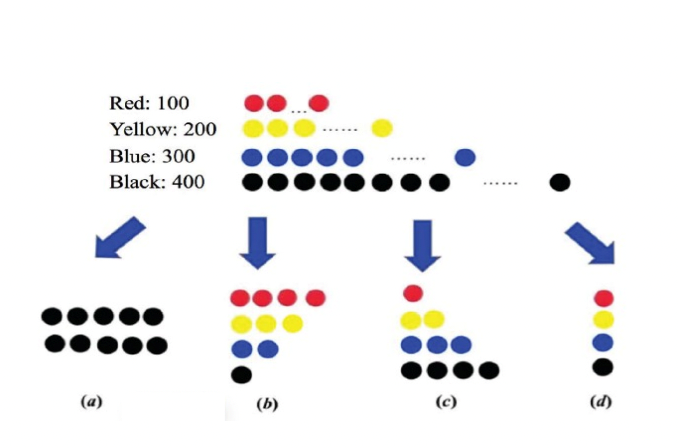
\includegraphics[height=3cm]{pre03-imgs/1.png}
            \end{figure}
        \end{minipage}\hspace{1cm}
        \medskip
        \begin{minipage}{0.5\linewidth}
            \begin{table}[ht]
                \centering
                \caption{结构覆盖度计算结果}
                \begin{tabular}{ccccc}
                    \toprule
                    度量指标 & a & b & c & d \\
                    \midrule
                    $\Cov_s^\text{range}$ & 0 & \textbf{0.625} & 1 & \textbf{0.7} \\
                    $\Cov_s^\text{var}$ & 0 & \textbf{0.9866} & 1 & \textbf{0.9833} \\
                    $\Cov_s$ & 0 & 0.8 & 1 & 0.923 \\
                    \bottomrule
                \end{tabular}
            \end{table}
        \end{minipage}

        \begin{itemize}
            \item 两种度量方法都能在结构覆盖度角度上选出c最能代表大数据集
            \item 在b和d的结构覆盖度的排序上,两种度量方法出现了差异
        \end{itemize}
    \end{frame}

    \section{冗余性度量}
    \begin{frame}
        \frametitle{冗余性度量}

        原文中使用了相似性这一概念来衡量集合中任意两个元素之间的可替代性(即在语义层面上互相间的代表性)。原文中并没有明确给出对于何种数据使用何样的相似性进行计算,但对于常见的如余弦相似性等相似度其本身往往具有轮换对称性。该性质在一般情况下自相似性语义角度来考虑是合理的,但是若是自语义的信息量角度来考虑便可以提出不对称的相似性定义,即本文所提出的冗余性(redundancy)。

    \end{frame}

    \begin{frame}
        \frametitle{冗余性度量}

        考虑对于评论数据集$D$场景下,存在两条评论$x, y$,其分别表达了不同消费者对于某件商品相似态度的语义,即二者表达了类似的语义,如同时对某件商品给出了正向的评论。若是评论$y$中的语义包含于评论$x$,即对于评论$x$,评论$y$并没有带来语义信息增益。相反,由于评论$x$的语义信息大于评论$y$,即评论$x$对于评论$y$带来了语义信息增益。

        我们使用了语义信息容量函数$G_S$来表达这一概念,其定义在集合$S$上,某一集合$X$在语义上能够反映大数据集合$S$中多少程度上的语义,其值域为$[0,1]$。显然有$G_S(S) = 1$与$G_S(\varnothing) = 0$。我们使用第一类冗余性(Redundancy Type I)的定义给出了对于大小数据问题下的冗余性的定义。

    \end{frame}

    \begin{frame}
        \frametitle{冗余性度量}

        对于$\forall x, y\in S$其冗余性函数为$r_S(x, y) = 1 - \left[G_S(\{x, y\}) - G_S(\{x\})\right]$,其表示了对于定义在集合$S$上的元素$x, y$,元素$y$相对于元素$x$的语义冗余。

        \begin{enumerate}
            \item 冗余函数$r_S(x, y)$的值域为$[0,1]$;
            \item 冗余函数$r_S(x, y)$不具备轮换对称性;
            \item 冗余函数$r_S(x, y)=0$当且仅当$G_S(\{y\}) = 1$。
            \item 冗余函数$r_S(x, y)=1$当且仅当$G_S(\{x, y\}) - G_S(\{x\}) = 0$ 。
        \end{enumerate}
    \end{frame}

    \begin{frame}
        \frametitle{冗余性度量}

        在此借助冗余度的概念,类似于原文中集合$D_j$的势给出基于冗余度的集合的势的概念,$n_j^\nu=\sum_{d\in D_j}{r_{D_j}(d_j^\prime,d)}$,其中$d_j^\prime$为集合$D_j$的类别标签。类似地给出$n^v=\sum_{j} n_j^v$,多样性的结构度量$\Cov_s(D^\prime,D)$同原文的计算方式。

        此处,我们给出一种冗余度函数的实例。

        \begin{equation}
            r_S\left(x,y\right)=1-\frac{1}{\left|S\right|}\sum_{d\in S}\left\{\max\left\{\Sim\left(x,d\right),\Sim\left(y,d\right)\right\}-\Sim\left(x,d\right)\right\} \label{eq:4}
        \end{equation}
    \end{frame}

    \begin{frame}
        \frametitle{冗余性度量计算}

        已知一组文档$d_i \in\{\textit{a,b,c,d,e,f}\}$,其相似度矩阵为$A = (\Sim(d_i, d_j))_{6\times 6}$:

        \begin{equation}
            A = \begin{bmatrix}
                1 & 0.95 & 0.03 & 0.05 & 0.12 & 0.21 \\
                0.95 & 1 & 0.13 & 0.08 & 0.15 & 0.01 \\
                0.03 & 0.13 & 1 & 0.87 & 0.92 & 0.78 \\
                0.05 & 0.08 & 0.87 & 1 & 0.85 & 0.95 \\
                0.12 & 0.15 & 0.92 & 0.85 & 1 & 0.77 \\
                0.21 & 0.01 & 0.78 & 0.95 & 0.77 & 1 \\
            \end{bmatrix}
        \end{equation}

        计算$D$中各元素相互的的冗余性指标和抽样$D' = \{e, a\}$的结构性度量。

    \end{frame}

    \begin{frame}
        \frametitle{冗余性度量计算}

        \begin{equation}
            A' = \left(a'_{ij}\right)_{6\times 6} = \begin{bmatrix}
                1 & 0.965 & 0.473 & 0.457 & 0.478 & 0.485 \\
                0.958 & 1 & 0.467 & 0.450 & 0.472 & 0.478 \\
                0.702 & 0.702 & 1 & 0.947 & 0.968 & 0.920 \\
                0.697 & 0.697 & 0.958 & 1 & 0.943 & 0.965 \\
                0.729 & 0.720 & 0.982 & 0.945 & 1 & 0.930 \\
                0.712 & 0.712 & 0.918 & 0.952 & 0.915 & 1 \\
            \end{bmatrix}
        \end{equation}

    \end{frame}

    \begin{frame}
        \frametitle{冗余性度量计算}

        分别使用$\Cov_s, \Cov_s^{\text{range}}, \Cov_s^{\text{var}}, \Cov_s^r$计算得到表\ref{tbl:2}

    \begin{table}[ht]
        \centering
        \caption{不同指标下的结构相似度}
        \begin{tabular}{cc}
            \toprule
            结构性度量指标 & 结构相似度 \\
            \midrule
            $\Cov_s$ & 0.99971 \\
            $\Cov_s^{\text{range}}$ & 0.97996 \\
            $\Cov_s^{\text{var}}$ & 0.9998 \\
            $\Cov_s^r$ & 0.9224 \\
            \bottomrule
        \end{tabular}
        \label{tbl:2}
    \end{table}

    \end{frame}

    \section{总结}
    \begin{frame}
        \frametitle{总结}

        综合来看,本文在Ma等人所提出的多样性结构度量的基础上进行了分析与改进,主要的工作内容有以下几点:

        \begin{enumerate}
            \item 本文分析了Ma等人提出的基于信息熵的多样性结构度量指标的合理性及其如何反应整体的信息结构;
            \item 本文在Ma等人的基础上,提出了基于方差与极差指标的结构性度量并论证了一些基本性质,最后给出了简单的例子计算二者与原基于信息熵结构度量指标的异同;
            \item 本文受Holst等人的启发,提出了基于第一类冗余定义的冗余度及其改进的势和多样性的结构度量,同样在简单的例子上进行了计算,并比较其与原文中结构度量指标的异同;
        \end{enumerate}

    \end{frame}
\end{document}